\documentclass[12pt]{kiarticle}
\graphicspath{{pictures/}}
\DeclareGraphicsExtensions{.pdf,.png,.jpg,.eps}
%%%
\pagestyle{fancy}
\fancyhf{}
%\renewcommand{\headrulewidth}{ 0.1mm }
\renewcommand{\footrulewidth}{ .0em }
\fancyfoot[C]{\texttt{\textemdash~\thepage~\textemdash}}
\fancyhead[L]{Вопрос по выбору --- ГКЭ, 2019\hfil}
\fancyhead[R]{\hfil Иванов Кирилл, 625 группа }
\usepackage{multirow} % Слияние строк в таблице
\newcommand
{\un}[1]
{\ensuremath{\text{#1}}}
\usepackage{tikz}
%%% Работа с таблицами
\usepackage{array,tabularx,tabulary,booktabs} % Дополнительная работа с таблицами
\usepackage{longtable}  % Длинные таблицы
\usepackage{multirow} % Слияние строк в таблице

\begin{document}
	
	\begin{titlepage}
	\begin{center}
		\large 	Московский физико-технический институт \\
		(государственный университет) \\
		Факультет общей и прикладной физики \\
		\vspace{0.2cm}
		
		\vspace{4.5cm}
		\Large{Общая физика: ГКЭ \\ \vspace{0.2cm}
			Вопрос по выбору} \\ \vspace{0.2cm}
		\LARGE \textbf{Модовый состав лазерного излучения}
	\end{center}
	\vspace{2.3cm} \large
	
	\begin{center}
		Работу выполнил: \\
		Иванов Кирилл,
		625 группа
		\vspace{10mm}		
		
	\end{center}
	
	\begin{center} \vspace{60mm}
		г. Долгопрудный \\
		2019 год
	\end{center}
\end{titlepage}



\section{Введение}

\textbf{Лазер} ---  источник квазимонохроматического и узконаправленного высококогерентного потока излучения, работающий за счёт квантово-механического эффекта вынужденного (индуцированного) излучения.

Главными элементами лазера являются \textbf{оптический резонатор} и расположенная в нём \textbf{активная среда}, способная усиливать проходящее через неё излучение.

\begin{figure}[h!]
	\centering
	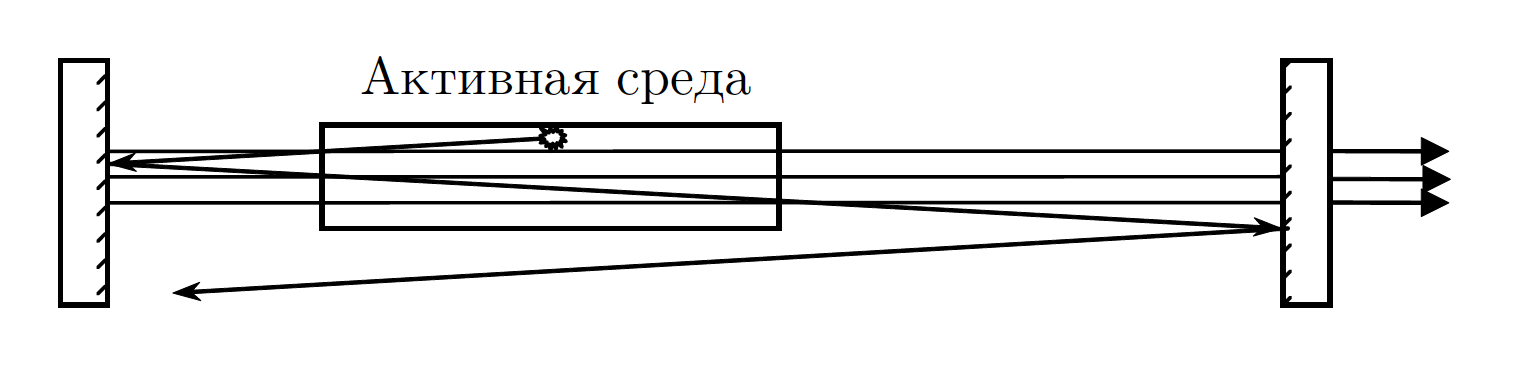
\includegraphics[width=0.7\linewidth]{laser.png}
	\caption{Схема лазера}
	\label{laser}
\end{figure}

\subsection{Квантово-механическое введение}

В силу выхода квантовой физики и связанных с ней явлений за рамки нашего курса мы не будем подробно останавливаться на квантово-механических принципах работы лазера.

Если вкратце, то из-за \textbf{спонтанного} (самопроизвольного) излучения электронами фотонов с энергией $ E = \hbar \omega $ появившиеся частицы света возбуждают атомы, заставляя их переходить на следующий энергетический уровень $ E_1 = E_0 + \hbar \omega $. После взаимодействия других фотонов с уже возбужденными электронами происходит \textbf{вынужденное} излучение, после чего атом возвращается в основное состояние. В результате этих процессов возникает электромагнитная волна с частотой $ \omega = \dfrac{E_1 - E_0}{\hbar} $, которая усиливается за счёт взаимодействия с активной средой.  

Конечно, нужно понимать, что в реальности такие волны являются не монохроматическими с бесконечно узкой линией поглощения/излучения $ \omega $, а обладают конечной шириной $ \Delta \omega $, которая называемся шириной спектра усиления активной среды лазера (\textbf{спектра генерации}). Она определяется из квантовых и иных характеристик атомов и активной среды.

Вывод показывает, что зависимость интенсивности излучения от частоты имеет форму гауссовой функции со спектром в интервале $ \omega \pm \Delta \omega $.

\subsection{Роль резонатора}

Простейший резонатор представляет собой \textbf{интерферометр
Фабри–Перо}, состоящий из двух плоских зеркал с
высокими коэффициентами отражения, размещённых параллельно друг другу на фиксированном расстоянии. Благодаря наличию
активной среды, в резонаторе многократно усиливаются волны, распространяющиеся вдоль оси системы и набирающие за один полный
проход резонатора фазу, кратную $ 2\pi $ (т.е. на оптической длине резонатора укладывается целое число полуволн, в системе при этом
образуются \textbf{стоячие волны}). Таким образом, резонатор обеспечивает
создание положительной обратной связи в лазере и превращает его
в генератор излучения. Также в резонаторе происходит накопление
энергии излучения и отбор узких резонансных линий из спектра
излучения, рождающегося в среде. Одно из зеркал резонатора обычно
имеет несколько меньший коэффициент отражения, что позволяет
выпускать через него часть излучения в виде узконаправленного
высокомонохроматического пучка.

\section{Модовый состав лазерного излучения}

\textbf{Модами} называют стационарные типы колебаний электромагнитного поля в резонаторе, различающиеся частотой и пространственным распределением амплитуды поля.

Рассмотрим моды в открытом резонаторе Фабри–Перо с плоскими
зеркалами, расстояние между которыми равно $ L $. Будем считать, для
простоты, что активная среда заполняет весь резонатор и имеет показатель преломления $ n= 1 $.

\subsection{Продольные моды}

Будем рассматривать \textbf{продольные моды}, т.е. волны, бегущие вдоль оси системы (пусть это будет $ x $). В результате отражения от зеркал мы получаем стоячие волны (см. рис. \ref{FP_waves}). Они задаются формулой $ E \propto \sin{\omega t} \sin{kx} $.

\begin{figure}[h!]
	\centering
	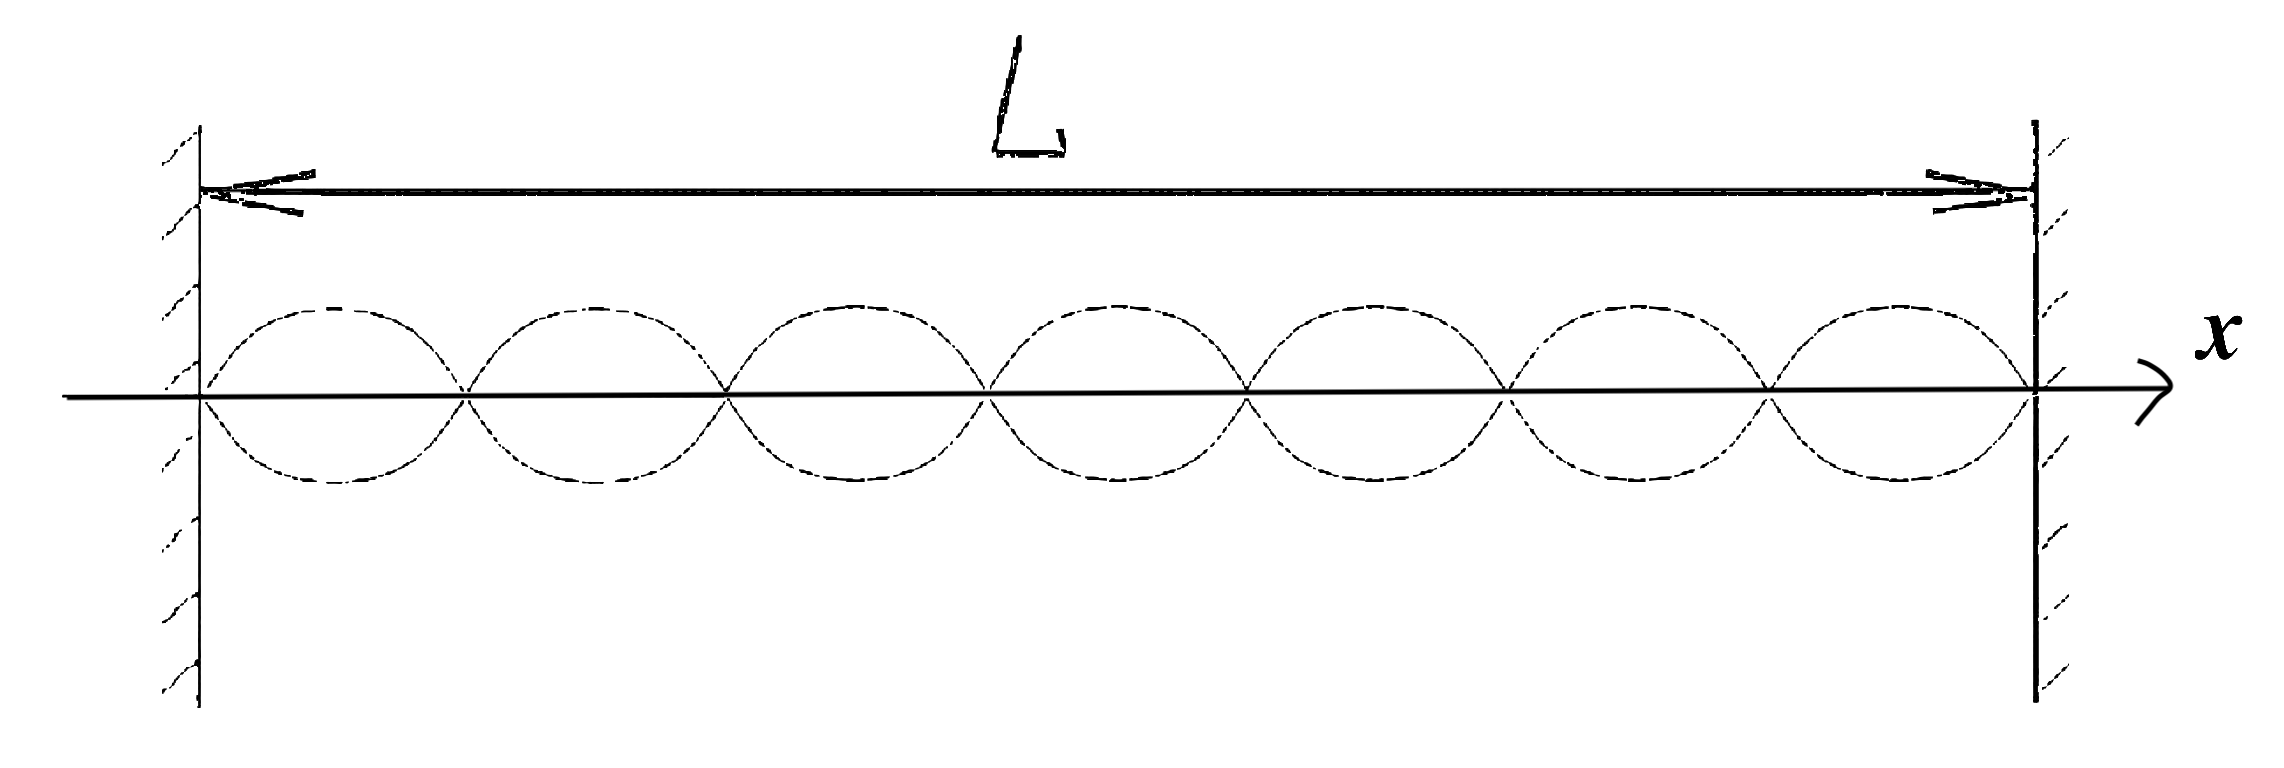
\includegraphics[width=0.7\linewidth]{FP_waves.png}
	\caption{Стоячие волны в плоскопараллельном резонаторе Фабри-Перо}
	\label{FP_waves}
\end{figure}

В случае металлических (проводящих) зеркал, электрическое поле на них (т.е. на границе системы, в точках $ x = 0, x = L $) обращается в ноль. Из этого условия и формулы выше мы получаем $ \sin{kx} = 0 \te kL =\pi m $, где $ m $, конечно же, пробегает значения $ m = 1, 2, 3, ... $ .  Подставляя волновое число $ k = \frac{2\pi}{\lambda} $, мы получаем условие на длину волны:

\begin{equation}\label{lamba/2}
\dfrac{\lambda}{2} = \dfrac{L}{m}
\end{equation}

Тогда нетрудно найти частоты, удовлетворяющие \eqref{lamba/2}. Так как частота световой волны $ \omega \hm{=} 2\pi \nu = 2 \pi \frac{c}{\lambda} $, получаем 

\begin{equation}\label{omega_m}
\omega_m = m \dfrac{\pi c}{L}
\end{equation}

Таким образом, мы получаем, что из всей ширины спектра генераций резонатор выделяет дискретный набор узких спектральных линий $ \omega_m $, соответствующих колебаниям продольных мод. Эти частоты также называются \textbf{собственными}. 

\subsection{Ширина спектральных линий}

\begin{wrapfigure}[13]{l}{0.45\linewidth} 
	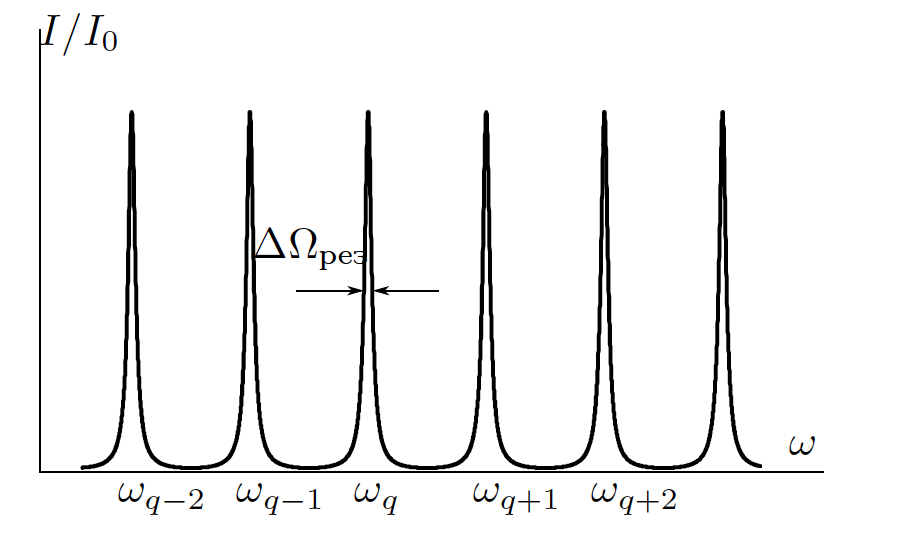
\includegraphics[width=\linewidth]{piks.png}
	\caption{Спектральная ширина собственных частот}
	\label{piks}
\end{wrapfigure}

Важно заметить, что эти линии не являются монохроматическими, а содержат в себе узкий спектр в интервале $ \omega_m \pm \Delta \Omega $, где полуширина резонансного пика $ \Delta \Omega $ согласно теории колебаний определяется через добротность системы: $ \Delta \Omega \hm{\sim} \dfrac{\omega_m}{Q} $. 

В силу определения добротности резонатора Фабри-Перо, мы получаем 

\begin{equation}\label{Q}
Q \sim \dfrac{2\pi L}{\lambda} \dfrac{1}{1 - \rho} \te \Delta \Omega \sim \dfrac{\omega_m}{Q}
\end{equation}

График распределения интенсивности мод от частоты представлен на рис. \ref{piks}. Заметим, что ввиду наличия усиления в активной среде, реальная ширина генерируемых лазером спектральных линий может быть
и значительно меньше полученной нами ширины линии пропускания резонатора. 

Обратим внимание на то, что из-за квантово-механических эффектов, а также в силу дифракции, поглощения и излучения существует такое понятие как \textbf{уровень потерь}. Помещая полученные нами спектральные линии под гауссову кривую, упомянутую в пункте 1.1, мы оставляем лишь те их них, которые больше этого уровня (рис. \ref{mods}).

\begin{figure}[h!]
	\centering
	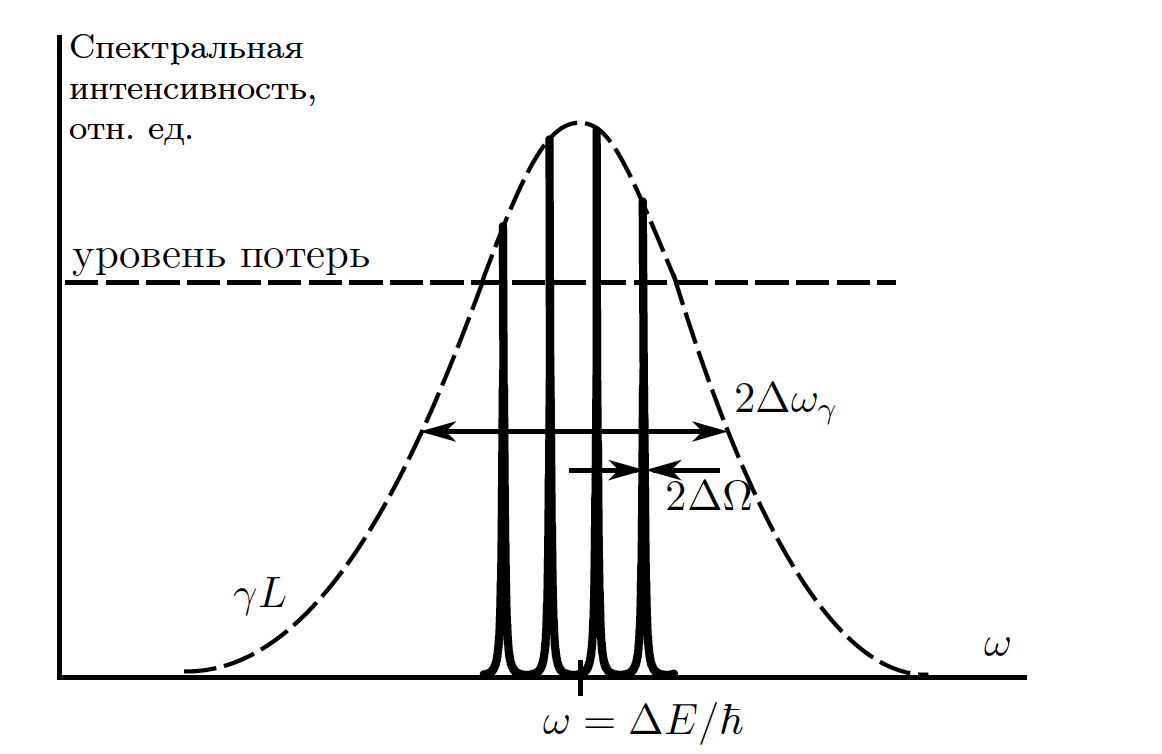
\includegraphics[width=0.7\linewidth]{mods.png}
	\caption{Многомодовый спектр излучения лазера}
	\label{mods}
\end{figure}

Такой спектр излучения лазера достаточно типичен и называется \textbf{многомодовым}. Количество генерируемых мод
зависит от соотношения усиления и потерь. Если усиление лишь немного выше уровня потерь, то возможна ситуация, когда будет возбуждена
только центральная линия и режим работы лазера будет \textbf{одномодовым}. Также одномодовый режим можно получить и иначе, о чем пойдет речь в дальнейшем.

\section{Экспериментальный подсчет числа мод}

Используем результаты выполненной в семестре \textbf{лабораторной работы № 4.5.2 ("<Интерференция лазерного излучения">)} для экспериментальной оценки числа продольных мод в гелий-неоновом лазере с длиной резонатора порядка $ 0,2 \divisionsymbol 1 $ м и средней длиной волны $ \lambda = 632,8 $ нм. 

Не вдаваясь в подробности лабораторной работы, объясним ее краткую суть (в части, интересной для нашего рассмотрения). С помощью экспериментальной установки мы расщепляем лазерное излучение и затем создаем между двумя полученными лучами геометрическую разность хода. Изучая зависимость видности интерференционной картины, которая задается формулой

\begin{equation}\label{V_2}
V_2 = \dfrac{1}{N} \dfrac{\sin {\frac{\pi l}{2L}N}}{\sin {\frac{\pi l}{2L}}},
\end{equation}

от разности хода $ l $, мы находим базу интерферометра $ L $ как расстояние $ 2L $ между двумя главными максимумами картины.  Из полученных в лабораторной данных построим график зависимости видности от разности хода.

\begin{figure}[h!]
	\centering
	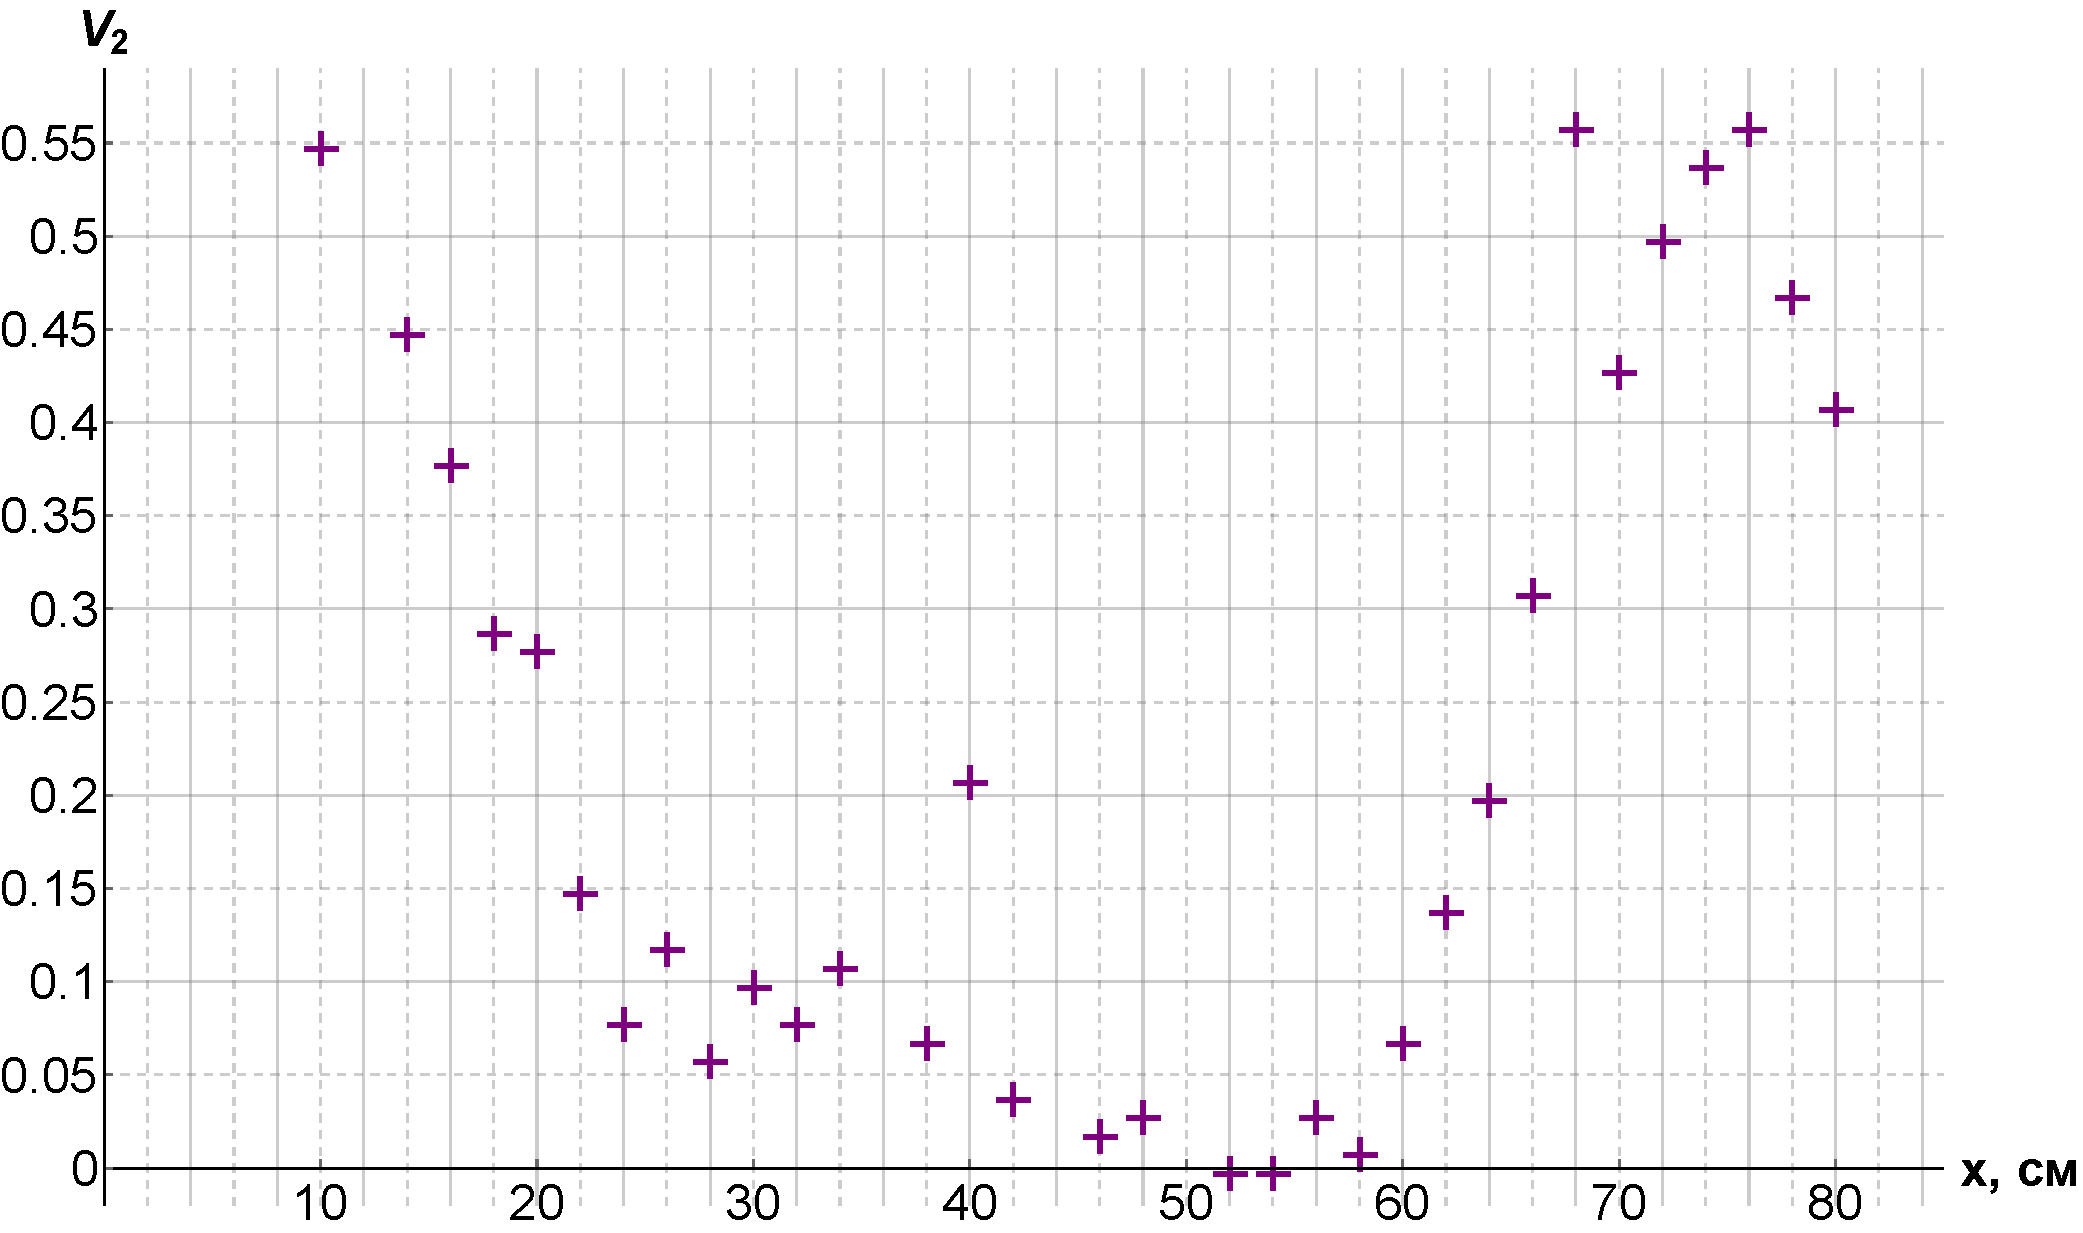
\includegraphics[width=0.9\linewidth]{V2.pdf}
	\caption{Экспериментальный график видности интерференционный картины лазера}
	\label{V2}
\end{figure}

Видно, что у нас наблюдается 2 максимума по краям области измерения и некоторые колебания в промежуточной области. А именно, максимумы в области $ x_1 \approx (10 \pm 2) \; см $ и в области $ x_2 \approx (75 \pm 2) \; см $, откуда получаем следующий результат:

\begin{equation}\label{}
L = \dfrac{1}{2} (x_2 - x_1) = (32,5 \pm 1,4) \; см
\end{equation}

Отсюда нетрудно получить и значение $ \Delta \nu $ --- расстояние между модами. 

\begin{equation}\label{delta nu}
\Delta \nu = \nu_{m+1} - \nu_m = \dfrac{с}{2L} \approx (4,6 \pm 0,2) \x 10^8 \; Гц
\end{equation}

Кроме того, при уменьшении видности картины в 2 раза мы можем замерить соответствующую координату $ l_{1/2} $ и подсчитать время когерентности $ \tau_к = l_{1/2}/c $. Тогда из принципа неопределённости $ \tau_к \Delta f \sim 1 $ мы можем получить ширину спектра генерации $ \Delta f = \frac{\Delta \omega}{2 \pi} $. С учетом более точного анализа кривых, определяемых \eqref{V_2}, можно уточнить формулу для $ \Delta f $ и получить интересующую нас формулу подсчета числа мод в виде

\begin{equation}\label{delta f}
\Delta f \approx 0,6 \dfrac{c}{l_{1/2}}, \qquad N \approx 1 + \dfrac{\Delta f}{\Delta \nu} = 1 + 1,2 \dfrac{L}{l_{1/2}}
\end{equation}

Оценим $ l_{1/2} \approx 18 - 10 = 8 \pm 2 $ см, откуда по формуле \eqref{delta f} получаем 

\begin{equation}\label{}
\Delta  f = 0,6\dfrac{c}{l_{1/2}} \approx (22,5 \pm 5,6) \x 10^8 \; Гц
\end{equation}

Тогда для числа генерируемых лазером продольных мод можно провести оценку:

\begin{center}
	{\fbox{$ N \approx 1 + 1,2 \dfrac{L}{l_{1/2}} \approx 6 \pm 1 $}} \\
\end{center} 

Такой результат вполне соотносится со типовыми показателями многомодовых гелий-неоновых лазеров.  

Попробуем проверить, кстати, как соотносятся расстояние между модами $ \Delta \omega_m = 2\pi  \Delta \nu_m \hm{\approx} 28,9 \x 10^8 \; с^{-1}$ и ширина резонансного пика. Оценив добротность системы по формуле \eqref{Q} и частоту резонансного пика из \eqref{omega_m} (полагая $ m \sim 10^7 $ для лазеров такого типа), мы получаем 

\begin{equation}\label{delta Omega}
Q \simeq 3,2 \x 10^8, \quad \omega_m \simeq 2,9 \x 10^{16} \; с^{-1} \te \Delta \Omega \simeq 0,9 \x 10^8 \; с^{-1}
\end{equation}

Видно, что исследуемые частоты отличаются на порядок. Все полученные величины хорошо соответствуют стандартным техническим характеристикам лазеров.

\section{Селекция продольных мод}

Зададимся вопросом селекции продольных мод, т.е. установлением \textbf{одномодового} режима работы лазера. 

Как мы говорили выше, расстояние между модами задается формулой \eqref{delta nu}. Понятно, что если $ \Delta \nu > \Delta f/2$, то у нас останется только одна мода. Этого можно достичь при использовании короткого резонатора с малым значением $ L $. Математически это условие формулируется неравенством

\begin{equation}\label{L < c/df}
L \leq \dfrac{c}{\Delta f}
\end{equation}

Например, расчёт для случая, полученного в пункте выше, будет составлять $ L \leq 13,3 $ см. Однако для многих типов лазера с большей шириной спектра генерации (например, твердотельных) необходимая длина будет слишком мала (миллиметры или даже меньше), что крайне тяжело реализовать на практике. Поэтому мы рассмотрим следующий оптический метод.

\subsection{Эталон Фабри-Перо для селекции продольных мод}

Обычно селекция продольных мод осуществляется путем размещения внутри резонатора одного или нескольких интерферометров Фабри-Перо, которые состоят из плоскопараллельной пластины из прозрачного материала. 

\begin{wrapfigure}[15]{l}{0.5\linewidth} 
	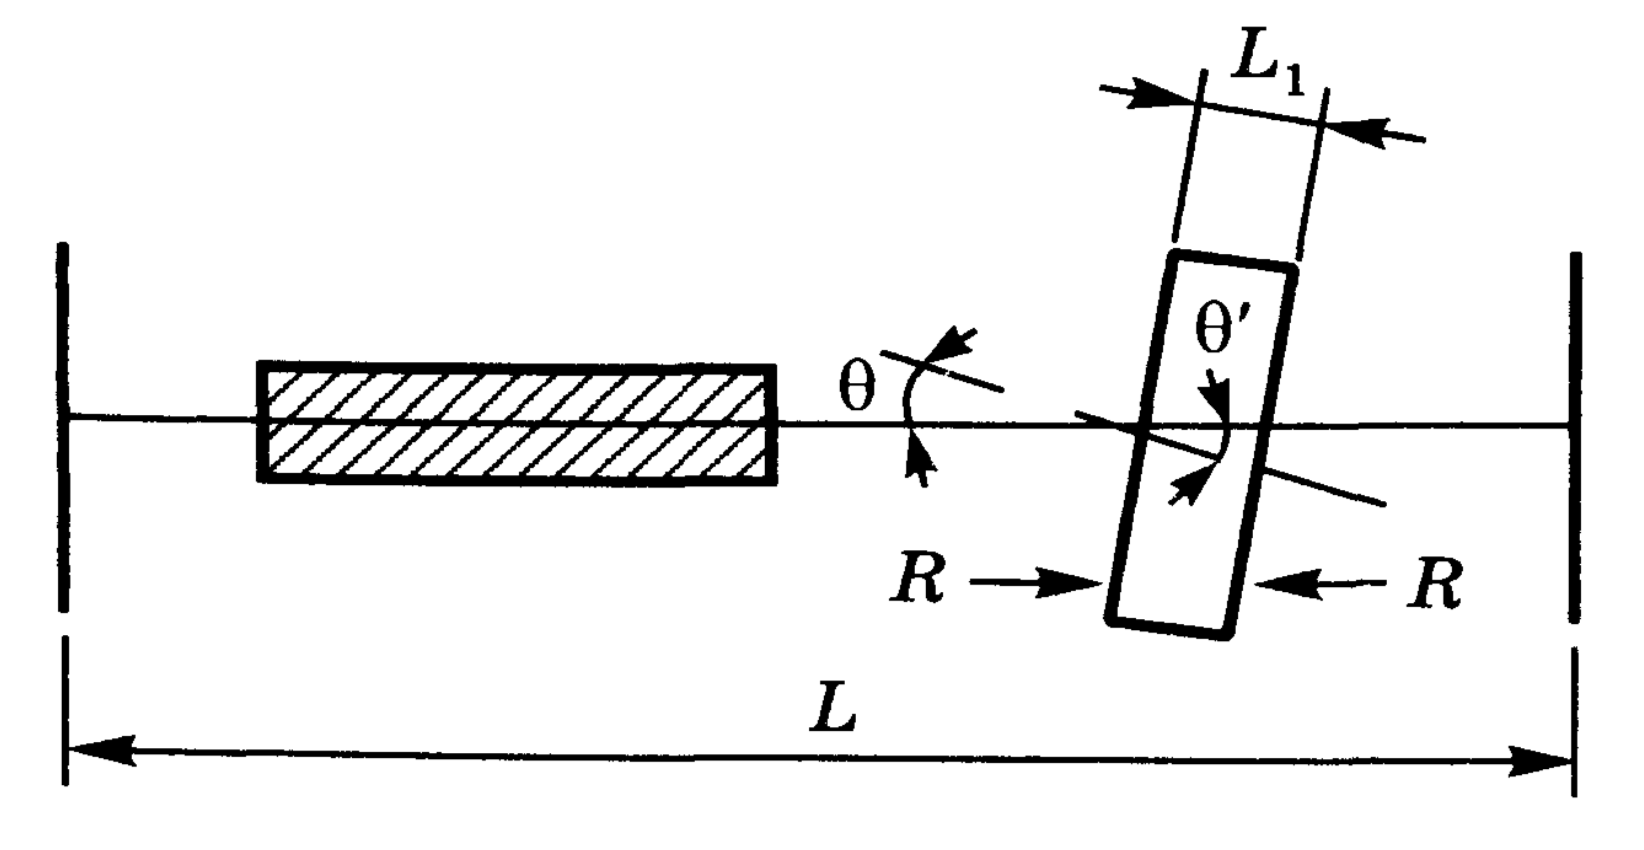
\includegraphics[width=\linewidth]{FP_selection}
	\caption{Схема для селекции продольных мод, использующая эталон 	Фабри-Перо, работающий на пропускание.}
	\label{FP_selection}
\end{wrapfigure}

Рассмотрим случай, когда в резонаторе используется один эталон Фабри-Перо, наклонённый под углом $ \theta $ к оси резонатора (рис. \ref{FP_selection}). В соответствии с формулой \eqref{omega_m}, максимумы этого эталона можно найти как 

\begin{equation}\label{}
\nu_m = m \dfrac{c}{2L_1 \cos \theta'}
\end{equation}

Поскольку $ L_1 $ намного меньше длины резонатора $ L $, в этом случае очень небольшого изменения угла $ \theta $ (и $ \theta' $) будет достаточно, чтобы настроить максимум пропускания эталона на центральную частоту контура усиления лазера. Понятно также, что т.к. все величины частот $ \nu \propto \frac{1}{L} $, то частотные характеристики эталона больше аналогичных для изначального резонатора. 

Если теперь наложить на расстояние между модами резонатора $ \Delta \nu $ условие, что оно больше полуширины пика эталона $ \Delta \nu_c $, то мы получаем следующий результат --- пик пропускания эталона оставляет лишь одну моду изначального резонатора, т.е. он селектирует ее. Наглядная картинка представлена на рис. \ref{selection}. 

\begin{figure}[h!]
 	\centering
 	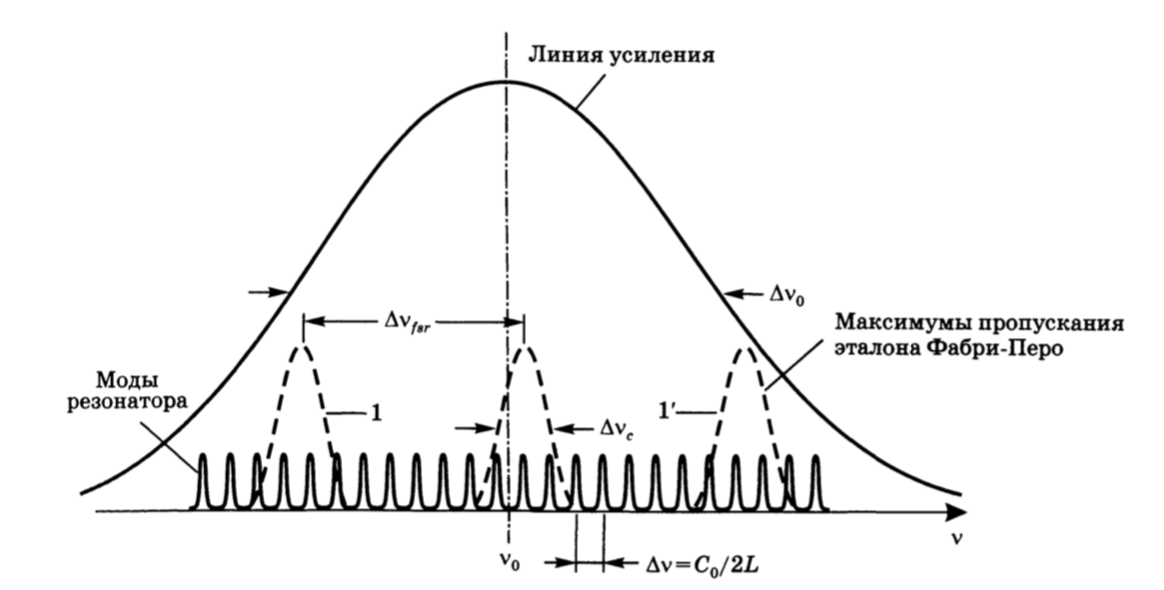
\includegraphics[width=0.7\linewidth]{selection}
 	\caption{{\small Максимумы пропускания эталонов, наложенные на обычное модовое излучение лазера}}
 	\label{selection}
\end{figure}

Введем характеристику "<\textbf{резкость}"> эталона $ F = \frac{\Delta \nu_f}{\Delta \nu_c} $ --- аналог добротности, который связывает расстояние между пиками $ \Delta \nu_f $ с их шириной $ \Delta \nu_c $. Тогда сформулированное выше условие мы запишем как

\begin{equation}\label{delta nu > delta nu_c/2}
\Delta \nu \geq \dfrac{\Delta \nu_c}{2} = \dfrac{\Delta \nu_f}{2F}
\end{equation}

Так мы уменьшаем число продольных мод излучения лазера до числа пиков эталона, которые находятся внутри гауссовой кривой линии усиления. Чтобы сократить это число до единицы, нам, очевидно, нужно оставить лишь один максимум пропускания эталона внутри диапазона $ \Delta f $. Это условие формулируется в виде $ \Delta \nu_f \geq \Delta f /2$. Совместно с \eqref{delta nu > delta nu_c/2}  мы получаем следующее:

\begin{equation}\label{}
2 F \Delta \nu \geq \Delta \nu_f \geq \dfrac{\Delta f}{2} \te 2 F \Delta \nu \geq \dfrac{\Delta f}{2}
\end{equation}

Подставляя значение $ \Delta \nu = \frac{c}{2L} $, мы получаем итоговый результат для длины резонатора $ L $:

\begin{equation}\label{}
L \leq 2F \dfrac{c}{\Delta f}
\end{equation}

Сравнивая это неравенство с \eqref{L < c/df}, мы замечаем, что ограничение на длину резонатора увеличилось в $ 2F $ раз. Стандартное значение резкости эталона Фабри-Перо $ F \sim 30 $. В самом деле, посмотрев, например, на наши результаты \eqref{delta Omega} из лабораторной работы, мы получаем $ F \approx \frac{28,9}{0,9} \simeq 32 $. \textbf{Т.е. один эталон дает возможность увеличить длину резонатора примерно в 60 раз}. 

Часто может не получиться оставить лишь одну моду с использованием одного эталона. В таком случае применяют два из них разной толщины. При использовании двух эталонов для разделения соседних продольных мод резонатора задействуется эталон, имеющий большее значение толщины.Второй, более тонкий эталон должен разделять соседние максимумы пропускания первого эталона. В таком случае, последовательно применяя вышеописанные рассуждения, мы получаем возможность увеличения до $ (2F)^2 $ раз. 

\section{Заключение}

Таким образом, мы изучили принципы работы лазеров и рассмотрели модовый состав их излучения (а именно, продольные моды). После теоретического описания многомодового режима работы мы экспериментально подсчитали основные характеристики модового спектра для гелий-неонового лазера с длиной резонатора 30 см и длиной волны 630 нм. 

Очень важен бывает вопрос о селекции мод, т.е. получение одномодового излучения лазера. Работать с таким практически монохроматическим светом намного удобнее, чем учитывать вклад нескольких различных мод. 
 Одним из популярных способов является использование эталонов Фабри-Перо внутри основного резонатора лазера. Это позволяет увеличивать длину резонатора при выделении одной продольной моды, что очень важно для практической реализации лазеров. 

\section*{Использованная литература}

\begin{itemize}
	
	\item Лабораторный практикум по общей физике: учеб. пособие. В трёх томах. Т. 2. Оптика / А.В. Максимычев, Д.А. Александров, Н.С. Берюлёва и др.; под ред. А.В. Максимычева. --- М.: МФТИ, 2014. --- 446 с.
	
	\item Звелто O "<Принципы лазеров/ Пер. под науч. ред. Т.А. Шмаонова. 4-е изд. --- СПб.: Издательство "<Лань">, 2008. --- 720 с.: ил. --- (Учебные пособия для вузов. Специальная литература).
	
\end{itemize}

\end{document}